\documentclass{../oxmathproblems}
\usepackage{blindtext}
\usepackage{hyperref}
\usepackage{geometry}

\course{ITAM - Estadística 1}
\oxfordterm{Assignment 01}
\sheetnumber{1}
\sheettitle{}

\extrawidth{2cm}

\begin{document}
\begin{questions}
\miquestion \textbf{Datos Cualitativos y distribuciones de frecuencia}

\begin{itemize}
\item  a) Cualitativo / Nominal 
\item  b) Cuantitativo / Razón
\item  c) Cualitativa / Nominal 
\item  d) Cuantitativa / Intervalo
\end{itemize}

\miquestion \textbf {Distribución de frecuencias y Diagrama de puntos}

\begin{itemize}
\item  a) Diagrama de barras: 
$$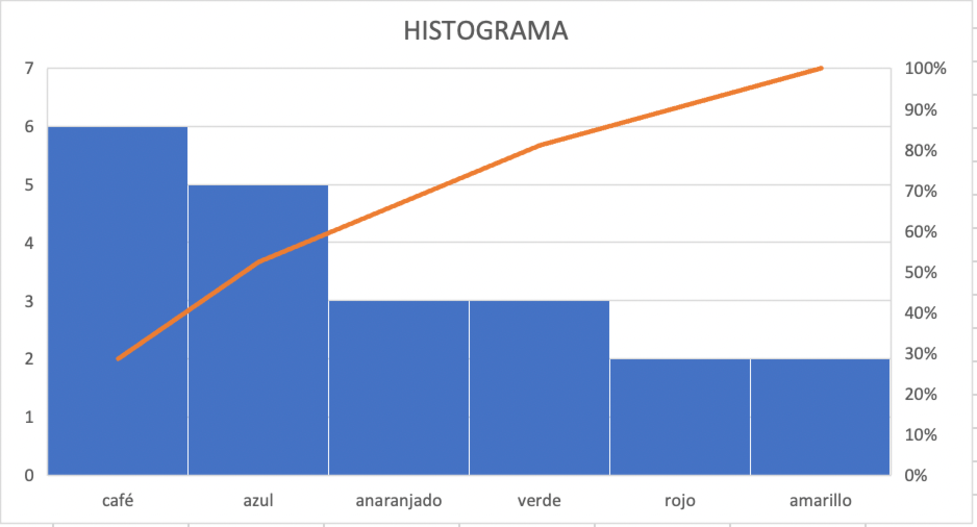
\includegraphics[width=0.8\textwidth]{A01-Histcolor}$$
\item  b) Diagrama de Puntos: 
$$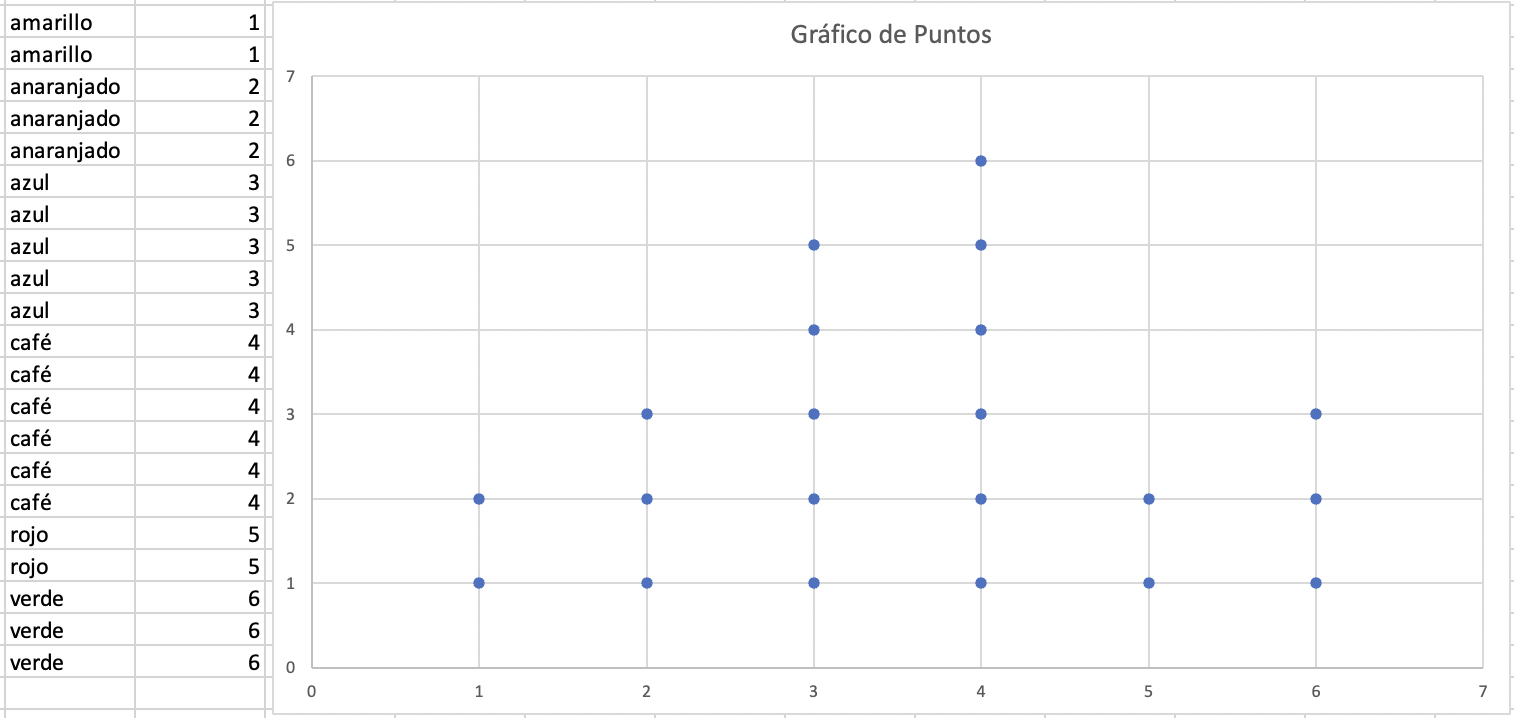
\includegraphics[width=0.8\textwidth]{A01-Diagramapunto}$$
\newpage
\item  c) Tabla de distribución de frecuencias: 
\begin{center}
\begin{tabular}{ |c|c|c|c|c|c|c|} 
\hline
Variable Cualitativa & Frec Absoluta & Frec Relativa & Frec Acumulada & Frec Acum Relat   \\
\hline
Amarillo &2 &0.095 & 2 & 0.095\\
Anaranjado &3& 0.143 & 5 & 0.238\\
Azul  & 5  & 0.238  & 10 & 0.476\\
Café & 6 & 0.286 &  16 &0.761\\
Rojo & 2 & 0.095 & 18 & 0.857\\
Verde & 3 & 0.143 & 21 & 1 \\
Total & 21 & 1 &- & - \\
\hline
\end{tabular}
\end{center}
\end{itemize}

\miquestion \textbf { Diagrama de Tallo y Hoja} 

4$\mid$ 0 

6$\mid$ 0 5 5 5 8 8 

7$\mid$ 0 0 0 0 0 0 0 

7$\mid$4  5 5 

9$\mid$ 0 5 

\text  {siendo} 9$\mid$ 0 \text  { como   90}


\miquestion \textbf { Variable Aleatoria Continua } 


\begin{itemize}
\item  a) Diagramas: 
$$\includegraphics[width=0.8\textwidth]{A04-Gráficos}$$
\item  b) Medidas de tendencia central y de dispersión: 
$$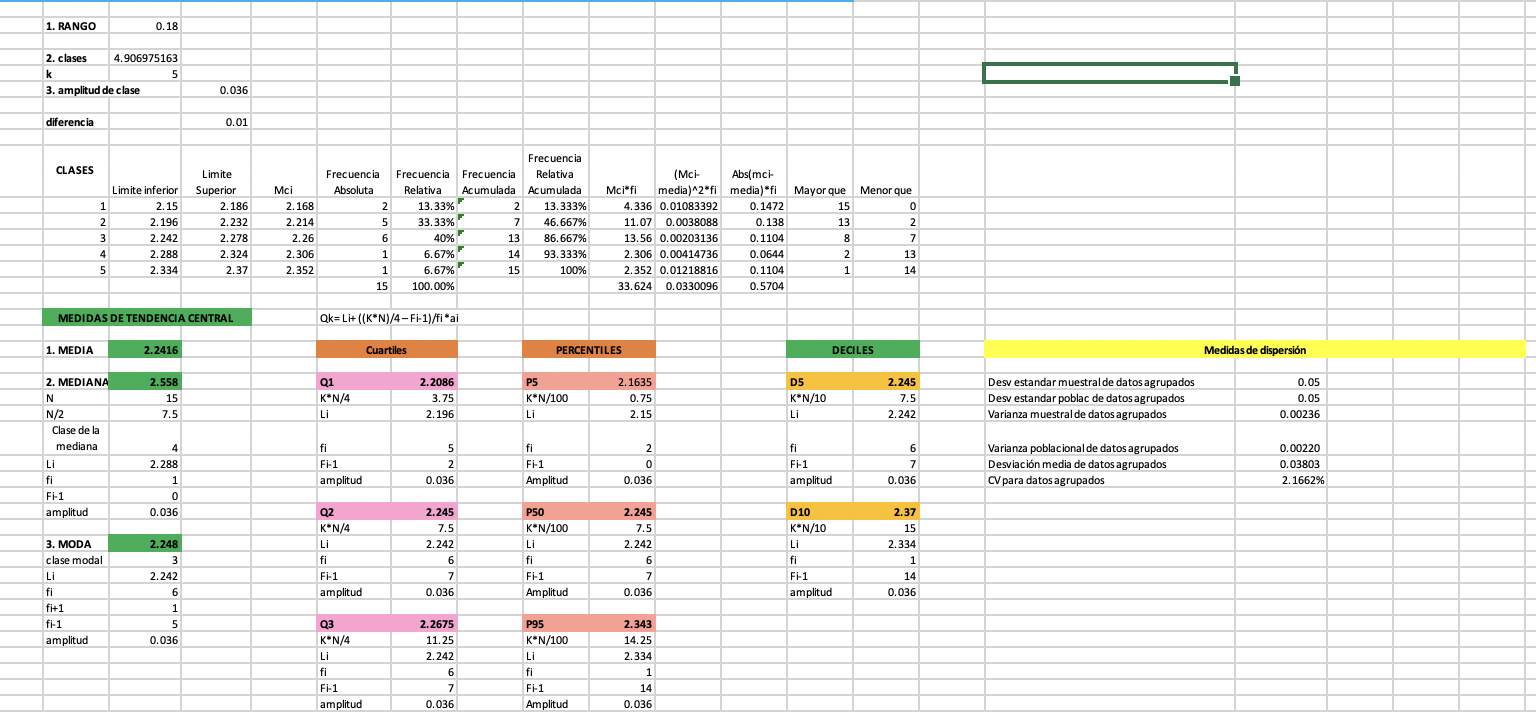
\includegraphics[width=0.8\textwidth]{A04-Medidasdedisp}$$
\end{itemize}

\end{questions}




\end{document}
